\documentclass[12pt]{article}
\usepackage{algo,fullpage,url,amssymb,epsfig,color,xspace,tikz,amsmath}
\usepackage{graphicx}
\usepackage{makecell}
\usepackage{float}
\usepackage[pdftitle={CS 486 Assignment 1},
pdfsubject={University of Waterloo, CS 486, Winter 2024},
pdfauthor={Arne Storjohann}]{hyperref}
\usepackage{algpseudocode,enumitem,calc,multicol}

\usepackage{listings}
\lstset{%
        language=python,
        keepspaces=true,
        basicstyle=\small\ttfamily,
       commentstyle=\footnotesize\itshape{},
       identifierstyle=\slshape{},
       keywordstyle=\bfseries,
       numbers=left,
       numberstyle=\tiny{},
       numberblanklines=false,
       inputencoding={utf8},
       columns=fullflexible,
       basewidth=.5em,
        fontadjust=true,
        tabsize=3,
        emptylines=*1,
       breaklines,
       breakindent=30pt,
        prebreak=\smash{\raisebox{-.5ex}{\hbox{\tiny$\hookleftarrow$}}},
    escapeinside={//*}{\^^M} % Allow to set labels and the like in comments starting with //*
	}

\renewcommand{\thesubsection}{Problem \arabic{subsection}}

\begin{document}

\begin{center}
  {\Large\bf University of Waterloo}\\ \vspace{3mm}
  {\Large\bf CS 486, Winter 2024}\\ \vspace{2mm}
  {\Large\bf Assignment 1}\\ \vspace{3mm}
\end{center}

\definecolor{care}{rgb}{0,0,0}
\def\question#1{\item[\bf #1.]}
\def\part#1{\item[\bf #1)]}
\newcommand{\pc}[1]{\mbox{\textbf{#1}}} % pseudocode

%%%%%%%%%%%%%%%%%%%%%%%%%%%%%%%%%%%%%%%%%%%%%
\subsection{} 
\begin{enumerate}
\part{a} 
	The Euclidean distance to the destination is an admissible heuristic function because it never overestimates the actual shortest path cost, as the shortest possible path between two cities is the straight line (Euclidean) distance between them, thus the only possible case is the Euclidean distance equals or \textbf{underestimates} the shortest path cost.

\part{b} 
	The Euclidean distance to the destination is a consistent heuristic function because it satisfies the monotone restriction: \textbf{heuristic estimate of the path cost is always less than or equal to the actual cost}. As previously stated the Euclidean distance could only equals or \textbf{underestimates} the shortest path cost.
	%\textbf{$h(n) -h(n) \le cost(m,n)$ for every arc $<m,n>$}

\part{c} Decision Tree:
	\begin{figure}[H]
	\center
	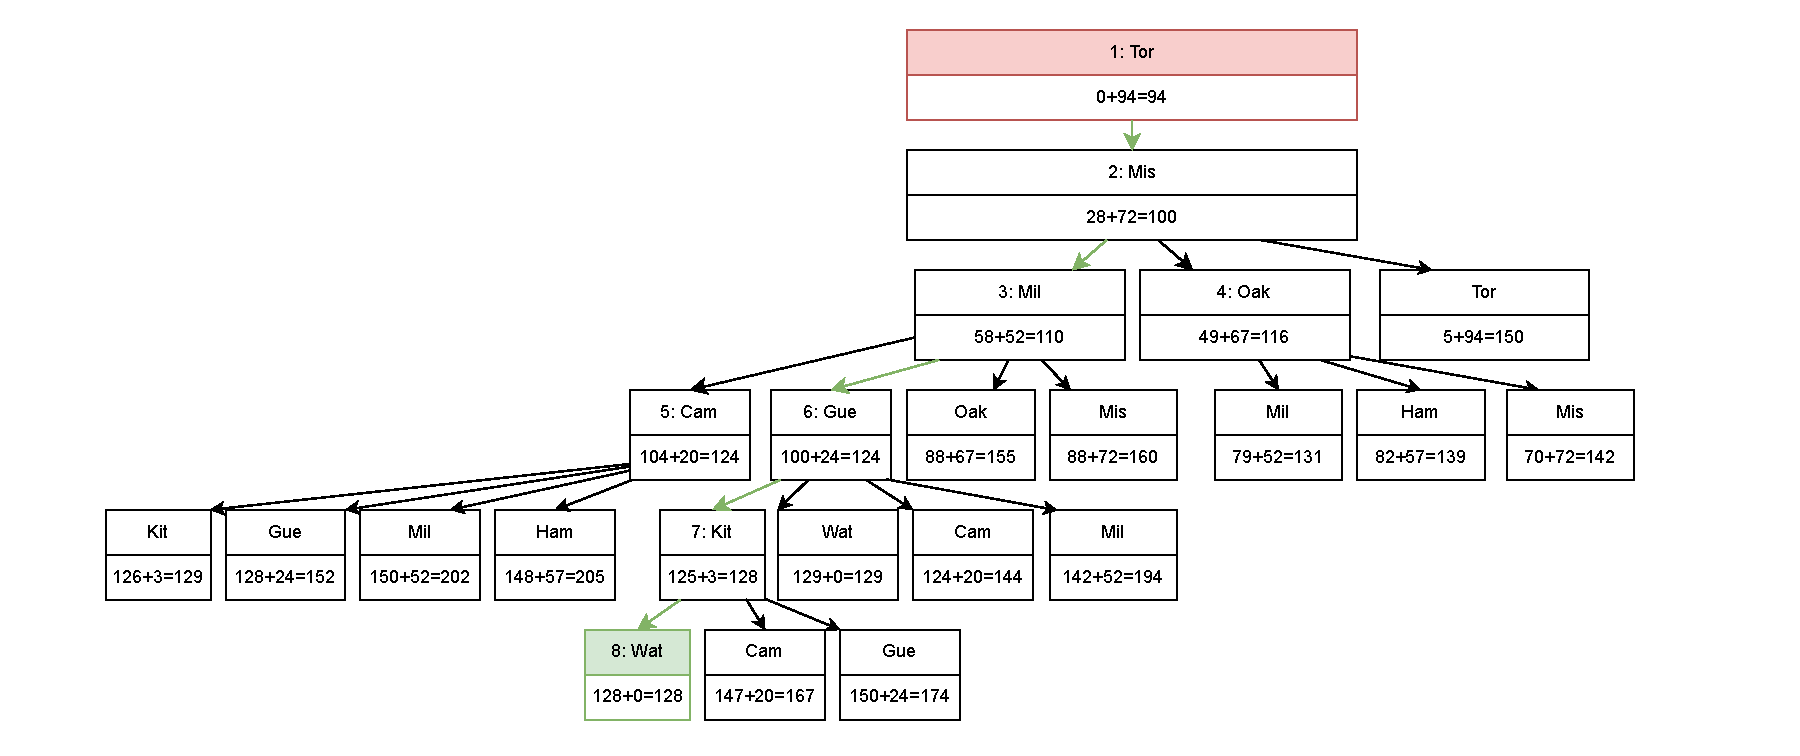
\includegraphics[width=18cm]{486A1Q1.pdf}
	\end{figure}

\end{enumerate}


%%%%%%%%%%%%%%%%%%%%%%%%%%%%%%%%%%%%%%%%%%%%%
%%%%%%%%%%%%%%%%%%%%%%%%%%%%%%%%%%%%%%%%%%%%%
\newpage
\subsection{} 
\begin{enumerate}

\part{a} \texttt{minimax}:

	\begin{lstlisting}
	if depth == 0 or node.state.is_terminal:
        # Base case: evaluate the state using the heuristic function
        node.value = heuristic_fn(node.state, max_role)
        return node.value
    if node.state.turn == max_role:
        # Maximizing player
        max_eval = float('-inf')
        for move in node.state.get_legal_moves():
            # Create a successor node
            successor_state = deepcopy(node.state)
            successor_state.advance_state(move)
            successor_node = MinimaxNode(successor_state)
            # Recursively call minimax on the successor
            eval = minimax(successor_node, depth - 1, max_role, heuristic_fn)
            # max_eval is the maximum evaluation value for the player.
            max_eval = max(max_eval, eval)
            # Store successor node and its value
            node.successors[move] = successor_node
        # Assign the maximum value found to the current node
        node.value = max_eval
        return max_eval
    else:
        # Minimizing player
        min_eval = float('inf')
        for move in node.state.get_legal_moves():
            # Create a successor node
            successor_state = deepcopy(node.state)
            successor_state.advance_state(move)
            successor_node = MinimaxNode(successor_state)
            # Recursively call minimax on the successor
            eval = minimax(successor_node, depth - 1, max_role, heuristic_fn)
            # min_eval is the minimum evaluation value for the player.
            min_eval = min(min_eval, eval)
            # Store successor node and its value
            node.successors[move] = successor_node
        # Assign the minimum value found to the current node
        node.value = min_eval
        return min_eval
	\end{lstlisting}\
	
\part{b} 
	
	The game always terminates in less than 10 seconds (around \texttt{0.04s} to \texttt{0.05s}) on my laptop for \texttt{RandomPlayer} vs. \texttt{MinimaxHeuristicPlayer} with depth \texttt{2}.
	
	The first depth number i encountered for the game not terminating within 10 seconds is \texttt{depth=6}, which takes around \texttt{34s} on my Laptop.

\part{c} 

	\texttt{my\_heuristic}:

	\begin{lstlisting}
	#If the state is terminal, give the true evaluation
    if state.is_terminal:
        if state.winner == '':
            return 0
        elif state.winner == max_role:
            return 100
        else:
            return -100
    #If the state is not terminal, give the heuristic evaluation
    score_board = [
        [1, 2, 3, 3, 2, 1],
        [2, 4, 6, 6, 4, 2],
        [3, 6, 9, 9, 6, 3],
        [4, 8, 12, 12, 8, 4],
        [3, 7, 10, 10, 7, 3],
        [2, 4, 6, 6, 4, 2],
        [1, 2, 3, 3, 2, 1],
        ]
    score = 0
    # Calculate the score for each piece based on its distance from the center column
    for col in range(state.num_cols):
        for row in range(state.num_rows):
            if state.board[col][row] == max_role:
                # Assign higher score to pieces closer to the center
                # The maximum score is given to the center column and decreases as it moves away from the center
                score += score_board[col][row]
            else:
                score -= score_board[col][row]
    return score
	\end{lstlisting}\
	
	\texttt{my\_heuristic} evaluates the board state by calculating a score based on the pieces' location on the board. Each spot on the board is given a score, with higher scores for spots closer to the centre. In the end, it returns the score as the difference between the total scores of the two players.
	
	I believe \texttt{my\_heuristic} will outperform \texttt{three\_line\_heur} because  my heuristic function assign scores based on board positions, more precisely based on the pieces' distance from the centre of the board. The closer a piece is to the centre, the higher its score, as closer a piece is to the centre, higher the chance that it will contribute to a connect-4, or stop a connect-4 attempt for the opponent. And \texttt{three\_line\_heur} only based scores on number of 3-in-a-row, without considering how easy is that 3-in-a-row to become an actual connect-4.  
		
\part{d} Diagram (each run 20 games):

	\begin{tabular}{|c|c|c|c|c|}
	\hline
 	Agent 1 & Agent 2 & Wins & Draws & Losses \\
	\hline
	\makecell{Minimax Player, depth 3 \\ three\_line\_heur} & RandomPlayer & 20 & 0 & 0 \\
	\hline
	\makecell{Minimax Player, depth 3 \\ my\_heuristic} & RandomPlayer & 20 & 0 & 0 \\
	\hline
	\makecell{Minimax Player, depth 5 \\ three\_line\_heur} & \makecell{Minimax Player, depth 2 \\ three\_line\_heur} & 16 & 1 & 3 \\
	\hline
 	\makecell{Minimax Player, depth 5 \\ my\_heuristic} & \makecell{Minimax Player, depth 2 \\ my\_heuristic} & 20 & 0 & 0 \\
	\hline
	\makecell{Minimax Player, depth 5 \\ my\_heuristic} & \makecell{Minimax Player, depth 5 \\ three\_line\_heur} & 15 & 0 & 5 \\
	\hline
	\end{tabular}

\end{enumerate}

%%%%%%%%%%%%%%%%%%%%%%%%%%%%%%%%%%%%%%%%%%%%%
%%%%%%%%%%%%%%%%%%%%%%%%%%%%%%%%%%%%%%%%%%%%%
\newpage
\subsection{} 
\begin{enumerate}
\part{1} 
	We will denote the $i$'th Queen's coordinate in the form $(X_i, Y_i)$. And the domain for them is $1 \le X_i \le N$ and $1 \le Y_i \le N$ for all $i \in \{1, 2, \dots, N\}$.
	
	And the constraints are:
	
	\begin{itemize}
		\item Row Constraint:
			$X_i \neq X_j $ for all  $i \neq j$ where $i,j \in \{1, 2, \dots, N\}$.
		
		\item Column Constraint:
			$Y_i \neq Y_j $ for all  $i \neq j$ where $i,j \in \{1, 2, \dots, N\}$.
			
		\item Diagonal Constraint: 
			$|X_i - X_j| \neq |Y_i - Y_j| $ for all  $i \neq j$ where $i,j \in \{1, 2, \dots, N\}$.

	\end{itemize}
		
\part{2} 
	We will denote the $i$'th Octopi's coordinate in the form $(X_i, Y_i)$. And the domain for them is $1 \le X_i \le N$ and $1 \le Y_i \le N$ for all $i \in \{1, 2, \dots, N\}$.
	
	And the constraints are:
	
	\begin{itemize}
		\item Row Constraint:
			$X_i \neq X_j $ for all  $i \neq j$ where $i,j \in \{1, 2, \dots, N\}$.
		
		\item Column Constraint:
			$Y_i \neq Y_j $ for all  $i \neq j$ where $i,j \in \{1, 2, \dots, N\}$.
			
		\item Block Constraint: 
			$\left\lfloor \frac{X_i - 1}{M} \right\rfloor \neq \left\lfloor \frac{X_j - 1}{M} \right\rfloor$ or $\left\lfloor \frac{Y_i - 1}{M} \right\rfloor \neq \left\lfloor \frac{Y_j - 1}{M} \right\rfloor$ for all  $i \neq j$ where $i,j \in \{1, 2, \dots, N\}$.


	\end{itemize}


\end{enumerate}

%%%%%%%%%%%%%%%%%%%%%%%%%%%%%%%%%%%%%%%%%%%%%
%%%%%%%%%%%%%%%%%%%%%%%%%%%%%%%%%%%%%%%%%%%%%

\end{document}
